\documentclass[a4paper,12pt]{article} 

%%% Работа с русским языком
\usepackage{cmap}                           % поиск в PDF
\usepackage{mathtext} 			 	       % русские буквы в формулах
\usepackage[T2A]{fontenc}               % кодировка
\usepackage[utf8]{inputenc}              % кодировка исходного текста
\usepackage[english,russian]{babel}  % локализация и переносы


\usepackage{wrapfig}


%Матеша
\usepackage{amsmath,amsfonts,amssymb,amsthm,mathtools} % AMS
\usepackage{icomma} % "Умная" запятая

%\mathtoolsset{showonlyrefs=true} % Показывать номера только у тех формул, на которые есть \eqref{} в тексте.

%% Шрифты
\usepackage{euscript}	 % Шрифт Евклид
\usepackage{mathrsfs} % Красивый матшрифт

%% Свои команды
\DeclareMathOperator{\sgn}{\mathop{sgn}}

%% Перенос знаков в формулах (по Львовскому)
\newcommand*{\hm}[1]{#1\nobreak\discretionary{}
{\hbox{$\mathsurround=0pt #1$}}{}}



%%% Заголовок
\author{Злобина Вера Б02-002}
\title{Лабораторная работа 2.5.1

Измерение коэффициента поверхностного натяжения жидкости}
\date{\today}

\begin{document}


\maketitle 

\newpage 

\subparagraph*{Цель работы:} 1) измерение температурной зависимости  коэффициента поверхностного натяжения дистиллированной воды с использованием известного коэффициента поверхностного натяжения спирта;  2) определение полной поверхностной энергии  и теплоты, необходимой для изотермического образования единицы  поверхности жидкости  при различной температуре. 


\subparagraph*{В работе используются:}прибор  Ребиндера  с термостатом и микроманометром; исследуемые жидкости; стаканы.





Наличие поверхностного слоя приводит к различию давлений по разные стороны от искривленной границы раздела двух сред.  Для сферического пузырька с воздухом  внутри жидкости избыточное давление даётся формулой Лапласа:

\begin{equation}
\Delta P = P_{внутри}- P_{снаружи}=\frac{2\sigma}{r}, 
\end{equation}

где $\sigma$ -- коэффициент поверхностного натяжения, $P_{внутри}$ и $Р_{снаружи}$ -- давление внутри пузырька и снаружи, $r$ -- радиус кривизны поверхности раздела двух фаз. Эта формула лежит в основе предлагаемого метода определения коэффициента поверхностного натяжения жидкости. Измеряется давление $\Delta P$, необходимое для выталкивания в жидкость пузырька воздуха.



\subparagraph*{Экспериментальная установка.} Исследуемая жидкость (дистиллированная вода) наливается в сосуд В (Рис.1). Тестовая жидкость  (этиловый спирт) наливается  в сосуд Е.  При измерениях  колбы герметично закрываются  пробками.   Через одну из двух пробок  проходит полая металлическая игла С. Этой пробкой закрывается сосуд, в котором  проводятся измерения. Верхний конец иглы открыт в атмосферу, а нижний погружен в жидкость. Другой сосуд герметично закрывается второй пробкой. При создании достаточного  разряжения воздуха в колбе с иглой пузырьки воздуха начинают пробулькивать через жидкость. Поверхностное натяжение можно определить по величине разряжения $\Delta P$ (1), необходимого для прохождения пузырьков (при известном радиусе иглы).


Разряжение в системе создается с помощью аспиратора А. Кран $К_2$ разделяет две полости аспиратора. Верхняя полость при закрытом кране $К_2$  заполняется водой. Затем кран $К_2$ открывают и заполняют водой  нижнюю полость  аспиратора.  Разряжение воздуха создается в нижней полости  при открывании крана $К_1$, когда  вода вытекает из неё по каплям. В колбах В и С, соединённых трубками с нижней полостью аспиратора,  создается такое же пониженное давление. Разность давлений в полостях с разряженным воздухом и атмосферой измеряется спиртовым микроманометром.
Для стабилизации температуры исследуемой жидкости через рубашку D колбы В непрерывно прогоняется вода из термостата.


Обычно кончик иглы лишь касается поверхности жидкости, чтобы исключить влияние гидростатического давления столба жидкости. Однако при измерении температурной зависимости коэффициента поверхностного натяжения возникает ряд сложностей. Во-первых, большая теплопроводность металлической трубки приводит к тому, что температура на конце трубки заметно ниже, чем в глубине жидкости. Во-вторых, тепловое расширение поднимает уровень жидкости при увеличении температуры. 


Обе погрешности можно устранить, погрузив кончик трубки до самого дна. Полное давление, измеренное при этом микроманометром, $P = \Delta P + \rho g h$. Заметим, что $\rho g h$  от температуры практически не зависит. Величину  $\rho g h$ следует измерить двумя способами. Во-первых, замерить величину  $P_1 = \Delta P ^\prime$, когда кончик трубки только касается поверхности жидкости. Затем при этой же температуре опустить иглу до дна и замерить $P_2 = \rho g h  + \Delta P+ \Delta P ^{\prime\prime}$ ($\Delta P^\prime, \Delta P^{\prime\prime}$ -- давление Лапласа). Из-за  несжимаемости  жидкости можно положить $\Delta P^\prime= \Delta P^{\prime\prime} $ и тогда $\rho gh = P_2-P_1$. Во-вторых, при измерениях $P_1$ и $P_2$ замерить линейкой  глубину погружения иглы $h$. Это можно сделать, замеряя расстояние между верхним концом иглы и любой неподвижной частью прибора при положении иглы на поверхности и в глубине колбы.


\begin{figure} [h!]
	\centering 
	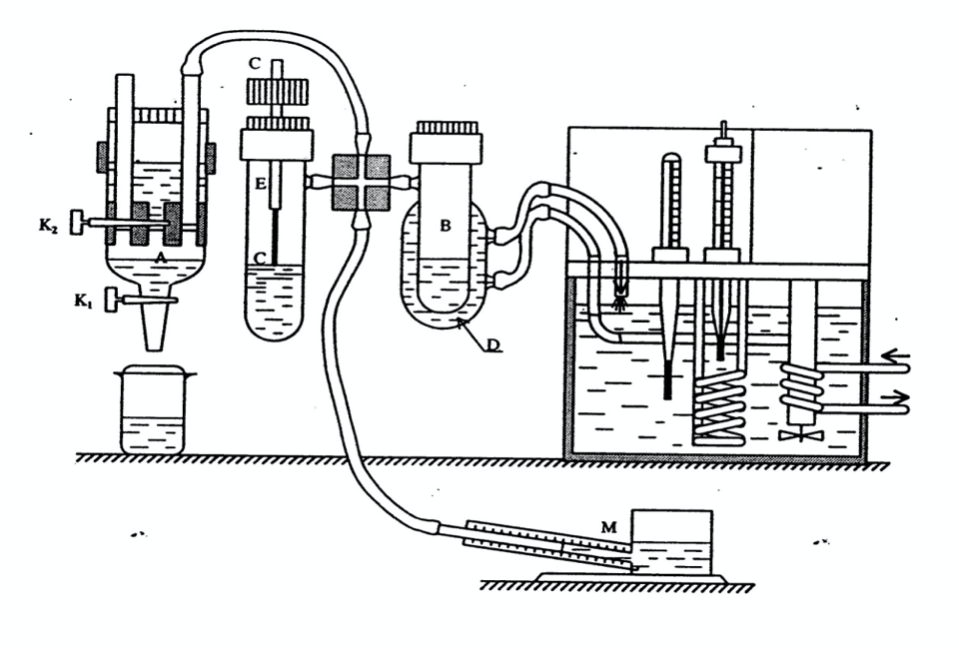
\includegraphics[scale=0.312]{1.jpg} 
	\caption{Схема установки} 
\end{figure}



\newpage

\section*{Ход работы}

\subparagraph{1.}Проверим герметичность установки. 

\subparagraph{2.} Откроем кран К1. Подберём частоту падения капель около одной капли в 5 секунд. 


\subparagraph{3.}  Измерим максимальное давление $\Delta P_{спирт}$  при  пробулькивании пузырьков воздуха через спирт. Данные занесём в Таблицу 1. По разбросу результатов оценим случайную погрешность измерения. 


\begin{table}[h!]
\centering
\caption{Измерения для спирта ($h_{сп}$)}
\begin{tabular}{|c|c|c|c|c|c|} \hline
 s& 1& 2 & 3& 4& 5 \\ \hline
 $h$, дел &47 & 48 & 47& 47& 47 \\ \hline
 \multicolumn{6}{|l|}{$h_{ср} = 47.2$ дел; $\sigma_h = 0.13$ дел} \\ \hline
 
\end{tabular}
\end{table}

В таблице учтена только случайная погрешность величины $h$, которая составляет около $0.3\%$  в то время как приборная погрешность составляет две цены деления (1 деление -- инструментальная погрешность и плюс ещё одно -- это моя реакция и способность зафиксировать правильное деление), то есть её относительный вклад $\approx 2 / 47 \approx 4.3\%$.

По формуле $\Delta P_{спирт} = 0.2 \cdot 9.81 \cdot h$ вычислим $\Delta P_{спирт}$.

$\Delta P_{спирт}  = (92.6\pm 4.0)~Па$


Пользуясь табличным значением коэффициента поверхностного натяжения спирта, определим по формуле (1) диаметр иглы. 


   	\begin{wrapfigure}{r}{0.27\linewidth} 
	\centering 
	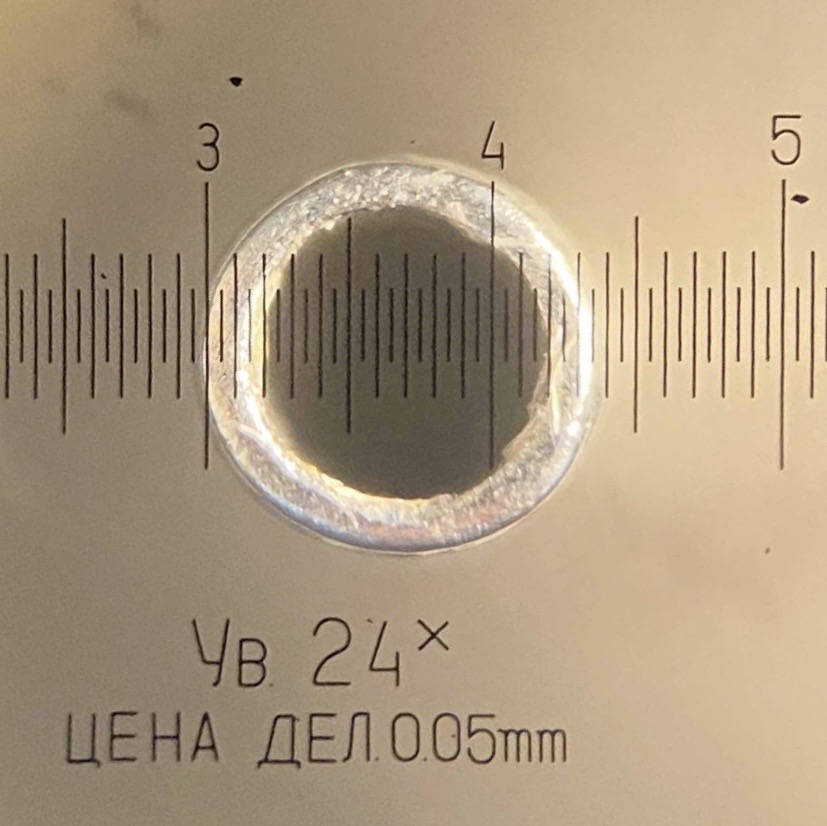
\includegraphics[scale=0.14]{контент.jpg} 
	\caption{Измерение диаметра иглы} 
\end{wrapfigure}

$
\sigma_{спирт, табл.} = 22,75 \cdot 10^{-3} ~  Дж /  м^2.
$


$
d_{рассч.}= \dfrac{4\sigma_{спирт, табл.}}{\Delta P_{спирт}}\approx 0.98~мм.
$

$
\dfrac{\sigma_d}{d}=\sqrt{\left(\dfrac{\sigma_{\Delta P}}{\Delta P}\right)^2}\approx 4.3\%.
$

Тогда итоговое значение 
$
d = (0.98 \pm 0.05)~ мм.
$

 Теперь воспользуемся микроскопом чтобы измерить диаметр иглы и сравним его с рассчитанным. Как проводились измерения можно увидеть на Рис. 2.
 
$
d_{изм} = (1.05 \pm 0.05)~ мм.
$

Здесь погрешность искомой величины определяется инструментальной погрешностью и равна цене деления, то есть 0.05 мм. 

Как видно, в пределах погрешности величины диаметра иглы совпали, что говорит о хорошо проведённых измерениях. 


\subparagraph{4.} Теперь перенесём иглу в колбу с водой, предварительно промыв её. Измерим максимальное давление $P_1$ при пробулькивании пузырьков, когда игла лишь касается поверхности воды. Отрегулируем скорость поднятия уровня спирта в манометре (около одной капли в 5 секунд) и будем сохранять её в течение всех экспериментов. 

\begin{table}[h!]
	\centering
	\caption{Измерения для воды ($h$)}
	\begin{tabular}{|c|c|c|c|c|c|} \hline
		s& 1& 2 & 3& 4& 5 \\ \hline
		$h$, дел &140 & 139 & 140& 140& 140 \\ \hline
		\multicolumn{6}{|l|}{$h_{ср} = 139.8$ дел; $\sigma_h = 0.13$ дел} \\ \hline
		
	\end{tabular}
\end{table}

Аналогично п.3 основной вклад в погрешность величины $h$ определяется инструментальной погрешностью, которая равна $\approx 2 / 139 \approx  1.5 \% $. Аналогично п.3 вычислим давление и в результате получим 

$
P_1 = (274.3 \pm 4.1) ~ Па.
$


Измерим расстояние между верхним концом иглы и любой неподвижной частью прибора $h_1$. Не забудем учесть инструментаальную погрешность железной линейки, равную 0.05 см.

$
h_1 = (1.85 \pm 0.05) ~ см.
$


\subparagraph*{5.} Утопим иглу до предела. Аналогично п.4 измерим $h_2$ и $P_2$.


\begin{table}[h!]
	\centering
	\caption{Измерение давления $P_2$}
	\begin{tabular}{|c|c|c|c|c|c|} \hline
		s& 1& 2 & 3& 4& 5 \\ \hline
		$h$, дел &204& 204& 204& 204& 204\\ \hline
    	\multicolumn{6}{|l|}{$h_{ср} = 204$ дел;}  \\ \hline
	\end{tabular}
\end{table}




$
P_2 = (400.2 \pm 3.9)~ Па.
$  

$
h_2 = (0.65 \pm 0.05)~ см.
$

По разности давлений $\Delta P= P_2 - P_1$ определим глубину погружения $\Delta h_1$ иглы и сравним с $\Delta h_2 =  h_1- h_2$. Погрешности при этом получаются по формулам $\frac{\sigma_{\Delta h_1} }{\Delta h_1}= \sqrt{\left(\frac{\sigma_{P_1}}{P_1}\right)^2 + \left(\frac{\sigma_{P_2}}{P_2}\right)^2}$ и $\frac{\sigma_{\Delta h_2} }{\Delta h_2}= \sqrt{\left(\frac{\sigma_{h_1}}{h_1}\right)^2 + \left(\frac{\sigma_{h_2}}{h_2}\right)^2}$



$
\Delta h_2 = h_1 - h_2 = (1.20 \pm 0.08)~ см
$

$
\Delta h_1 = \dfrac{P_1 - P_2}{\rho g} = (1.50 \pm 0.06)~см. 
$

Полученные значения для глубины погружения близки, но всё же не перекрываются погрешностью. Скорее всего расхождения обусловлены влиянием краевых эффектов, которое дало нам слегка завышенное значение  $P_2$. 


\subparagraph{6.} Снимем температурную зависимость $h (T)$ дистиллированной воды. Для этого включим термостат и подождём, пока нужная нам температура не стабилизируется. После этого проведём измерение давления. И так будем снимать показания через каждые 3 градуса. Результаты измерений занесены в Таблицу 4. 


\begin{table}[h!]
	\caption{Измерение давления в зависимости от температуры}
	\centering 
	\begin{tabular}{{|l}*{8}{|l}} \hline 
		$T,~^\circ С$ & \multicolumn{5}{c|}{$h, ~ дел$}& $h_{ср}, ~ дел $& $ \sigma_h, ~ дел$\\ \hline
		20.0 & 204 & 204 & 203 & 204 & 204 & 203.8 & 0.13 \\ \hline 
		24.2 & 203 & 203 & 203 & 204 & 203 & 203.2 & 0.13 \\ \hline
		26.6 & 203 & 203 & 203 & 202 & 203 & 202.8 & 0.13 \\ \hline 
		29.6 & 202 & 202 & 202 & 202 & 202 & 202.0 & 0.00 \\ \hline
		32.5 & 201 & 202 & 201 & 202 & 202 & 201.6 & 0.25 \\ \hline 
		35.5 & 201 & 201 & 200 & 201 & 201 & 200.8 & 0.13 \\ \hline
		38.5 & 200 & 200 & 200 & 199 & 200 & 199.8 & 0.13 \\ \hline 
		41.4 & 199 & 199 & 199 & 199 & 199 & 199.0 & 0.00 \\ \hline 
		44.3 & 198 & 198 & 198 & 197 & 198 & 197.8 & 0.13 \\ \hline 
		47.0 & 196 & 196 & 197 & 196 & 196 & 196.8 & 0.13  \\ \hline 
		50.3 & 195 & 195 & 195 & 195 & 195 & 195.0 & 0.00 \\ \hline 
		53.3 & 194 & 194 & 194 & 194 & 194 & 194.0 & 0.00 \\ \hline 
		56.0 & 193 & 194 & 194 & 193 & 194 & 193.6 & 0.25 \\ \hline 
		59.0 & 192 & 193 & 193 & 193 & 192 & 192.6 & 0.25 \\ \hline		
	\end{tabular}
\end{table}


\subparagraph*{7.} Оценим погрешность измерения давления и температуры. Для давления погрешность вычисляется аналогично п.3, а температура измерена с точностью около $0.2 ^\circ С$, что составляет около $0.1 \%$, поэтому данная погрешность учитываться не будет ввиду её малости.ассчитаем величину коэффициента поверхностного натяжения воды  $\sigma$, используя формулу, которая следует из (1): 

$$
\frac{\Delta P_{сп}}{\Delta P} = \frac{\sigma_{сп}}{\sigma} .
$$



Поскольку $P \propto h,$ то для вычисления $\sigma$ возьмём $h$ из Таблиц 1 и 2. При этом относительная погрешность величины $\sigma$  складывается из относительных погрешностей измерения давления: $\varepsilon_\sigma =\sqrt{\varepsilon_{h_1}^2 + \varepsilon_{h_2}^2} \approx 4.4 \%$, в результате чего получаем: 

$
\sigma = \sigma_{сп}\dfrac{h}{h_{сп}} \approx (68.4 \pm 3.0)\cdot 10^{-3} ~Дж /м^2.
$

 В то время как табличное значение коэффициента поверхностного натяжения воды при $25^\circ С$ составляет $71.8 \cdot 10^{-3} ~Дж /м^2, $ что почти перекрывается с полученным нами значением. 

\subparagraph*{8.}По данным Таблицы 4 построим график зависимости  $h(T)$ (Рис. 3).


\begin{figure} [h!]
	\centering 
	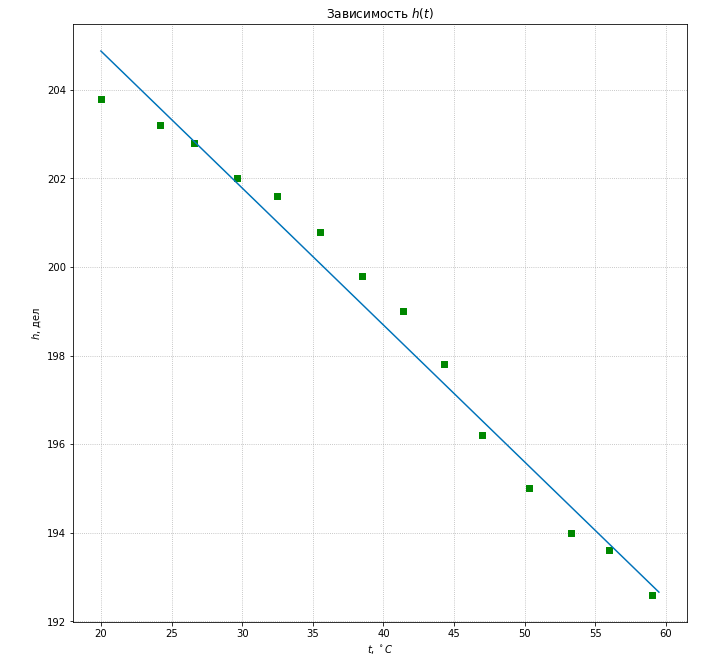
\includegraphics[scale=0.55]{2.jpg} 
	\caption{График, демонстрирующий измеренную зависимость давления от температуры} 
\end{figure}

Используя МНК определим коэффициент наклона $k = -0.31 ~ дел/~^\circ С$. 
 Определим по графику температурный коэффициент  $\alpha = - \dfrac{d\sigma}{dT} = -\dfrac{\sigma_{сп}}{h_{сп}}\cdot \dfrac{d h}{d T} = -\dfrac{\sigma_{сп}}{h_{сп}}\cdot k \approx 0.15 ~мДж / м^2 \cdot К$. Оценим точность результата. Пренебрежём погрешностью, вносимой инструментальной погрешностью термометра (почему это можно сделать описано ранее), поэтому итоговая погрешность величины складывается из погрешности, возникающей из-за аппроксимацией прямой (вычисляется по формуле из МНК $\sigma_k = \frac{1}{\sqrt{n}}\sqrt{\frac{\left< h^2\right>}{\left< t^2\right>} - k^2} \approx 0.04~мДж / м^2 \cdot К,$  то есть $\varepsilon_k =  12 \%$) Поскольку величина $h$ измерена с точностью не менее $4\%$ (по оценкам выше), то будем учитывать вклад только погрешности, возникающей из МНК. Тогда итоговый результат:
 
 $
\alpha  =( 1.49 \pm 0.18)  \cdot 10^{-4}~Дж / м^2 \cdot К.
 $
 
 Это значение перекрывается с табличным $1.54 \cdot 10^{-4} ~Дж / м^2\cdot К$ в пределах погрешности. 

\subparagraph*{9.}На других графиках построим зависимость от температуры 


а) теплоты образования единицы поверхности жидкости $q=-T\dfrac{d\sigma}{dt} = \alpha T$ (Рис. 4) 






б) поверхностной энергии $U$ единицы площади $F:   \dfrac{U}{F}= \sigma - T\dfrac{d\sigma}{dT}$ (Рис. 5). 









\newpage

\begin{figure}[h!]
	\centering 
	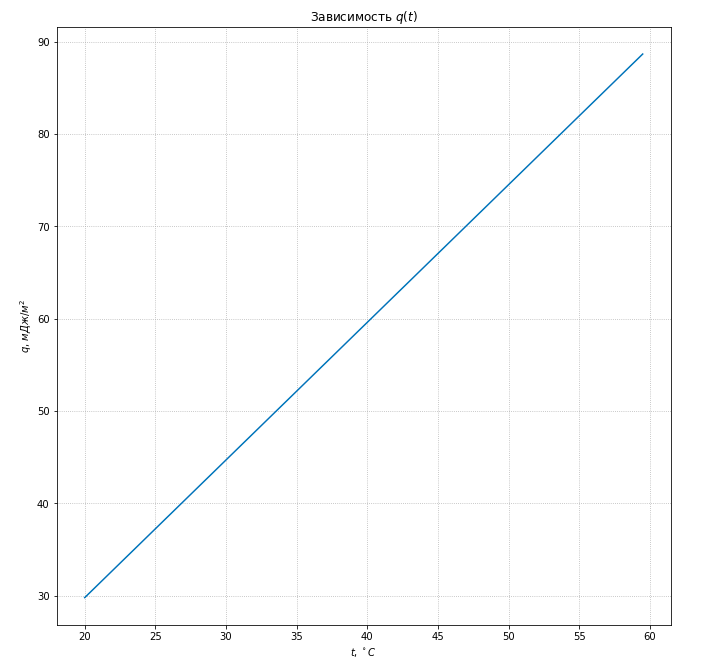
\includegraphics[scale=0.57]{3.jpg} 
	\caption{График зависимости теплоты образования единицы поверхности жидкости от температуры} 
\end{figure}

\newpage


\begin{figure} [h!]
	\centering 
	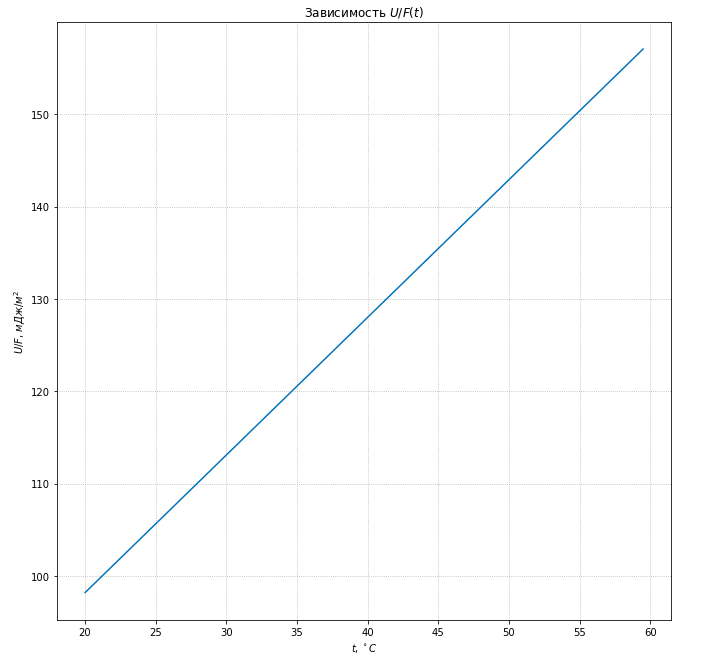
\includegraphics[scale=0.57]{4.jpg} 
	\caption{График зависимости поверхностной энергии $U$ единицы площади $F$ от температуры} 
\end{figure}



\newpage


\section*{Вывод}

В ходе работы был измерен коэффициент поверхностного натяжения воды, который почти совпал с табличным, так же было вычислено значение тепературного коэффициента поверхностного натяжения воды, которое уже совпало с табличным. Так же в ходе работы мы попробовали двумя способами измерить диаметр иглы, как выяснилось, если делать это с помощью косвенных измерений (сначала измерять разность давлений, а затем через неё и известный коэффициент поверхностного натяжения спирта вычился диаметр) то точность будет примерно такой же, если измерять диаметр напрямую с помощью микроскопа (относительная погрешность при этом около $5\%$. На самом деле стоило измерить диаметр с помощью микроскопа дважды: в двух поперечных направлениях и взять среднее, тогда может быть результаты совпали бы ещё точнее с рассчётными. Немного не сошлись результаты при проверке закона Паскаля: давление от разности высот, то есть $\rho g \Delta h$, оказалось несколько меньше, чем измеренная напрямую разность $P_1 - P_2$, я думаю это можно объяснить завышением давления в момент, когда игла только касается поверхности воды, тогда появляется давление из-за кривизны поверхности. 




\end{document}
